% $Header: /cvsroot/latex-beamer/latex-beamer/solutions/generic-talks/generic-ornate-15min-45min.en.tex,v 1.4 2004/10/07 20:53:08 tantau Exp $

\documentclass[10pt]{beamer}

\definecolor{verdfosc}{rgb}{0,0.2,0}


\newsavebox{\savepar}
\newenvironment{boxit}%
{\begin{lrbox}{\savepar}
  \begin{minipage}[b]{20cm}}
{\end{minipage}\end{lrbox}\fbox{\usebox{\savepar}}}


\newenvironment{quadre}[1]%
{\begin{center}\begin{lrbox}{\savepar}
  \begin{minipage}[b]{#1 cm}}
{\end{minipage}\end{lrbox}\fbox{\usebox{\savepar}}\end{center}}

\newenvironment{codi}[1]%
{\begin{small}
 \color{verdfosc}
 \begin{quadre}{#1}  
 

 }
{ 
  \end{quadre}
  \end{small} 
  \normalcolor
}




\mode<presentation>
{
  \usetheme{Warsaw}
  % or ...Warsaw Malmoe, Singapore, PaloAlto, Warsaw, Copenhagen

  \setbeamercovered{transparent}
  % or whatever (possibly just delete it)
}


\usepackage[english]{babel}
\usepackage[latin1]{inputenc}
\usepackage{color}
\usepackage{listings}
%Listings setup:
\definecolor{grey}{rgb}{0.8,0.8,0.8}

\lstloadlanguages{Java,XML}

\lstset{language=Java,
        numbers=left, 
        numberstyle=\footnotesize, 
        numbersep=7pt,
        frame=shadowbox, 
        framexleftmargin=5mm, 
        xleftmargin=0.6cm,
        rulesepcolor=\color{grey}
       }







%\usepackage{pstricks,pst-node,pst-tree}
%\usepackage{times}
%\usepackage[T1]{fontenc}
% Or whatever. Note that the encoding and the font should match. If T1
% does not look nice, try deleting the line with the fontenc.

\title[Zimbra 8 High Availability on Ubuntu 12.04]{Zimbra 8 High Availability on Ubuntu 12.04}

%\subtitle{Free as in freedom}

\author[Adri\'an Gibanel L\'opez] % (optional, use only with lots of authors)
{Adri\'an Gibanel L\'opez}
%{F.~Author\inst{1} \and S.~Another\inst{2}}
% - Use the \inst{?} command only if the authors have different
%   affiliation.

\institute[Universitat de Lleida] % (optional, but mostly needed)
{Universitat de Lleida}

%  \inst{1}%
%  Department of Computer Science\\
%  University of Somewhere
%  \and
%  \inst{2}%
%  Department of Theoretical Philosophy\\
%  University of Elsewhere}
% - Use the \inst command only if there are several affiliations.
% - Keep it simple, no one is interested in your street address.

\date[]{September 2013}

%\subject{Cooperative Game Theory}
% This is only inserted into the PDF information catalog. Can be left
% out. 



% If you have a file called "university-logo-filename.xxx", where xxx
% is a graphic format that can be processed by latex or pdflatex,
% resp., then you can add a logo as follows:

% \pgfdeclareimage[height=0.5cm]{university-logo}{university-logo-filename}
% \logo{\pgfuseimage{university-logo}}



% Delete this, if you do not want the table of contents to pop up at
% the beginning of each subsection:
\AtBeginSubsection[]
{
  \begin{frame}<beamer>
    \frametitle{Outline}
    \tableofcontents[currentsection,currentsubsection]
  \end{frame}
}


% If you wish to uncover everything in a step-wise fashion, uncomment
% the following command: 

%\beamerdefaultoverlayspecification{<+->}


\begin{document}

\definecolor{un}{rgb}{0.75,0,0}
\definecolor{dos}{cmyk}{0.95,0,0.5,0.3}
\definecolor{tres}{rgb}{0.85,0.75,0}
\definecolor{quatre}{rgb}{0.2,0.4,0.9}


\setbeamercolor{cyanBox}{fg=black,bg=cyan}

\begin{frame}
  \titlepage
\end{frame}


%\section*{Outline}
  \begin{frame}<beamer>
    \frametitle{Outline}
    \tableofcontents[section]
  \end{frame}


\section {Zimbra}
\begin{frame}
\frametitle{Zimbra Collaboration Server}


\begin{block}{}
Complete collaboration solution accessible from web client, offline clients and other emails and mobile devices
\end{block}


\quad

\begin{itemize}

\item Email
\item Address Book
\item Calendar
\item Tasks

\end{itemize}

\end{frame}

\begin{frame}
\frametitle{Zimbra Collaboration Server - Email}

\begin{center}
  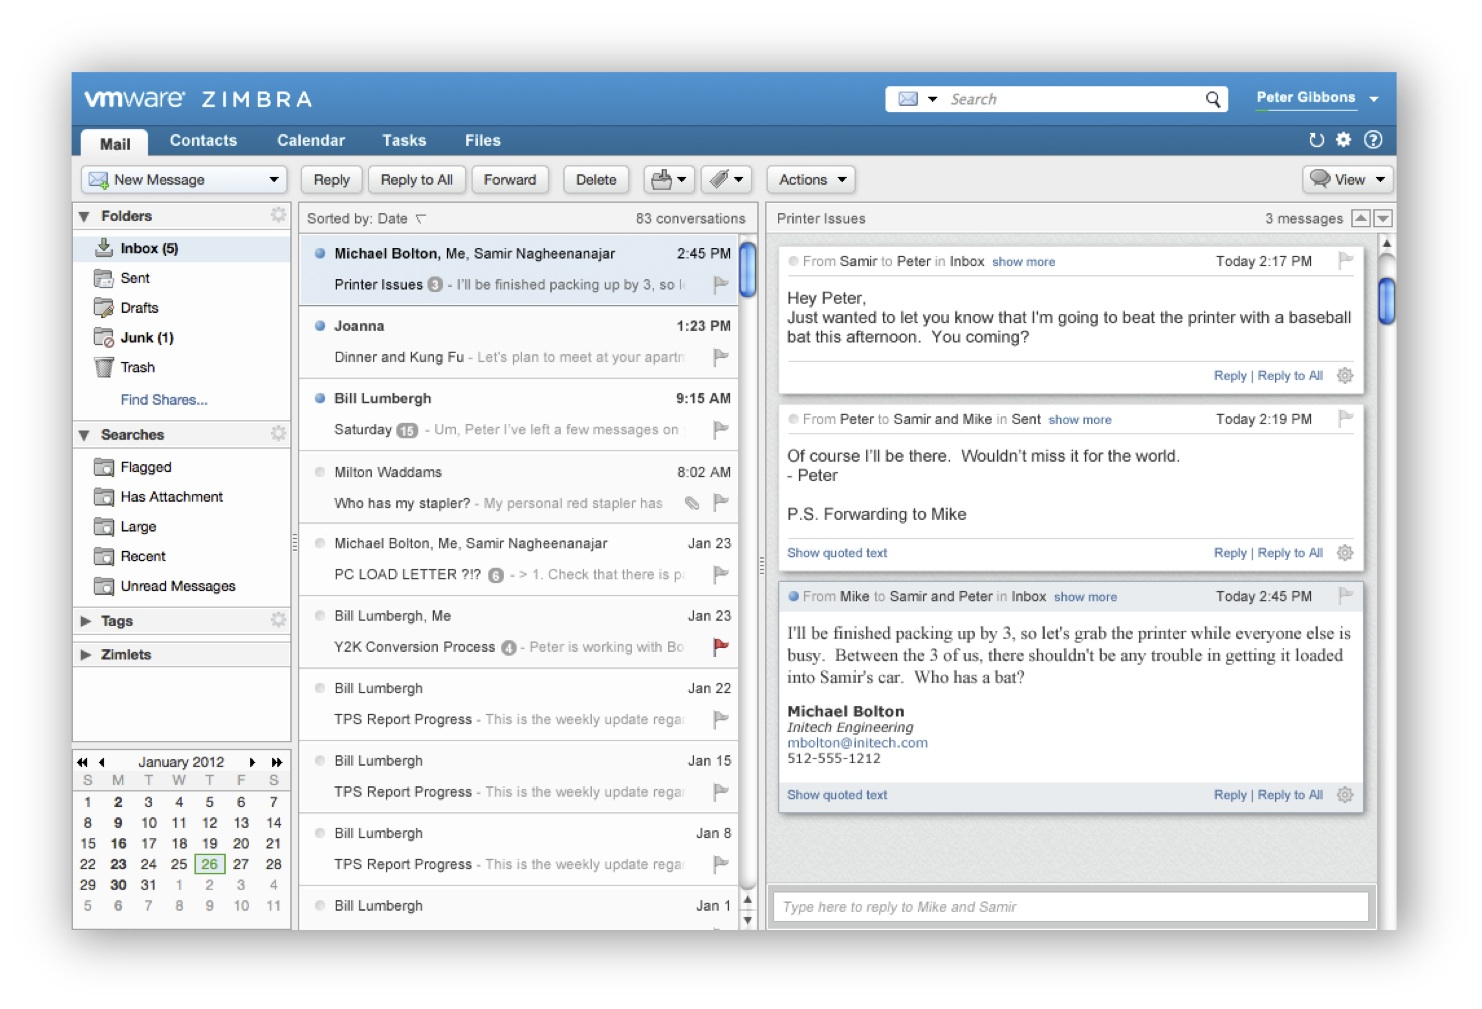
\includegraphics[scale=0.4,keepaspectratio=true]{./img/zimbra-email.jpg}
  % zimbra-email.jpg: 1482x1009 pixel, 150dpi, 25.10x17.09 cm, bb=0 0 711 484
\end{center}
\end{frame}

\begin{frame}
\frametitle{Zimbra Collaboration Server - Calendar}

\begin{center}
  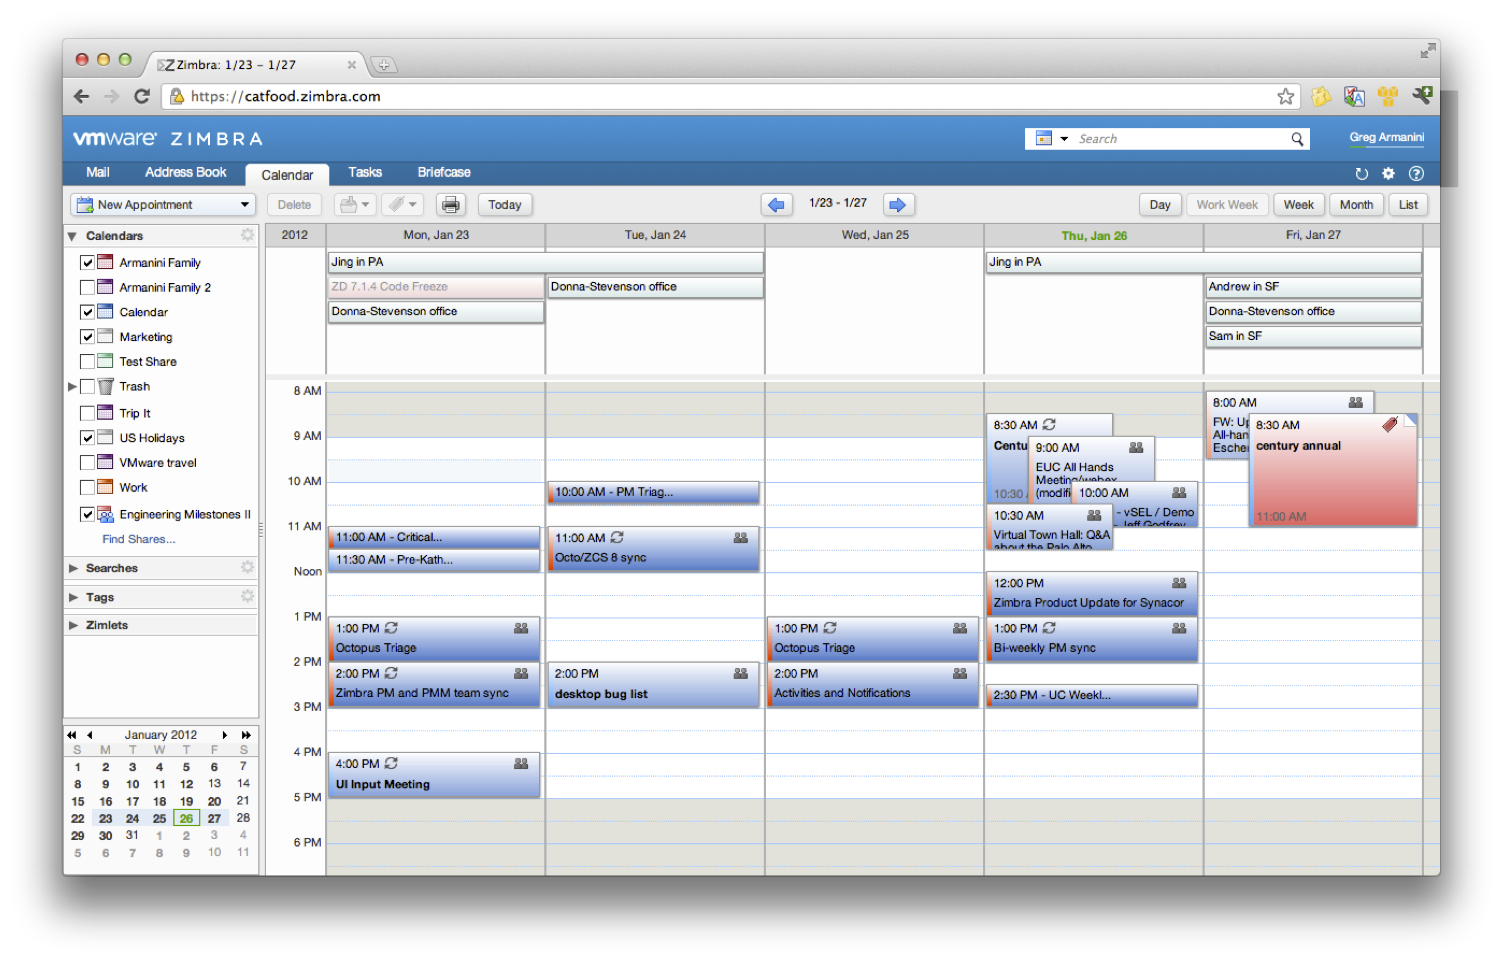
\includegraphics[scale=0.4,keepaspectratio=true]{./img/zimbra-calendar.jpg}
  % zimbra-calendar.jpg: 1503x961 pixel, 150dpi, 25.45x16.27 cm, bb=0 0 721 461
\end{center}


\end{frame}
\section {Zimbra High Availability}
\begin{frame}
\frametitle{ZCS High Availability}


\begin{block}{}
HA: System design approach that ensures that a prearranged level of operational performance will be met during a contractual measurement period.
\end{block}


\quad

\begin{itemize}

\item HA Active/Passive cluster for Zimbra
\item Minimize downtime due to Hardware or telecommunication failures
\item Minimal Zimbra modifications
\item Use of standard open source High Availability software

\end{itemize}

\end{frame}


\begin{frame}
\frametitle{ZCS HA Schema}

\begin{center}
  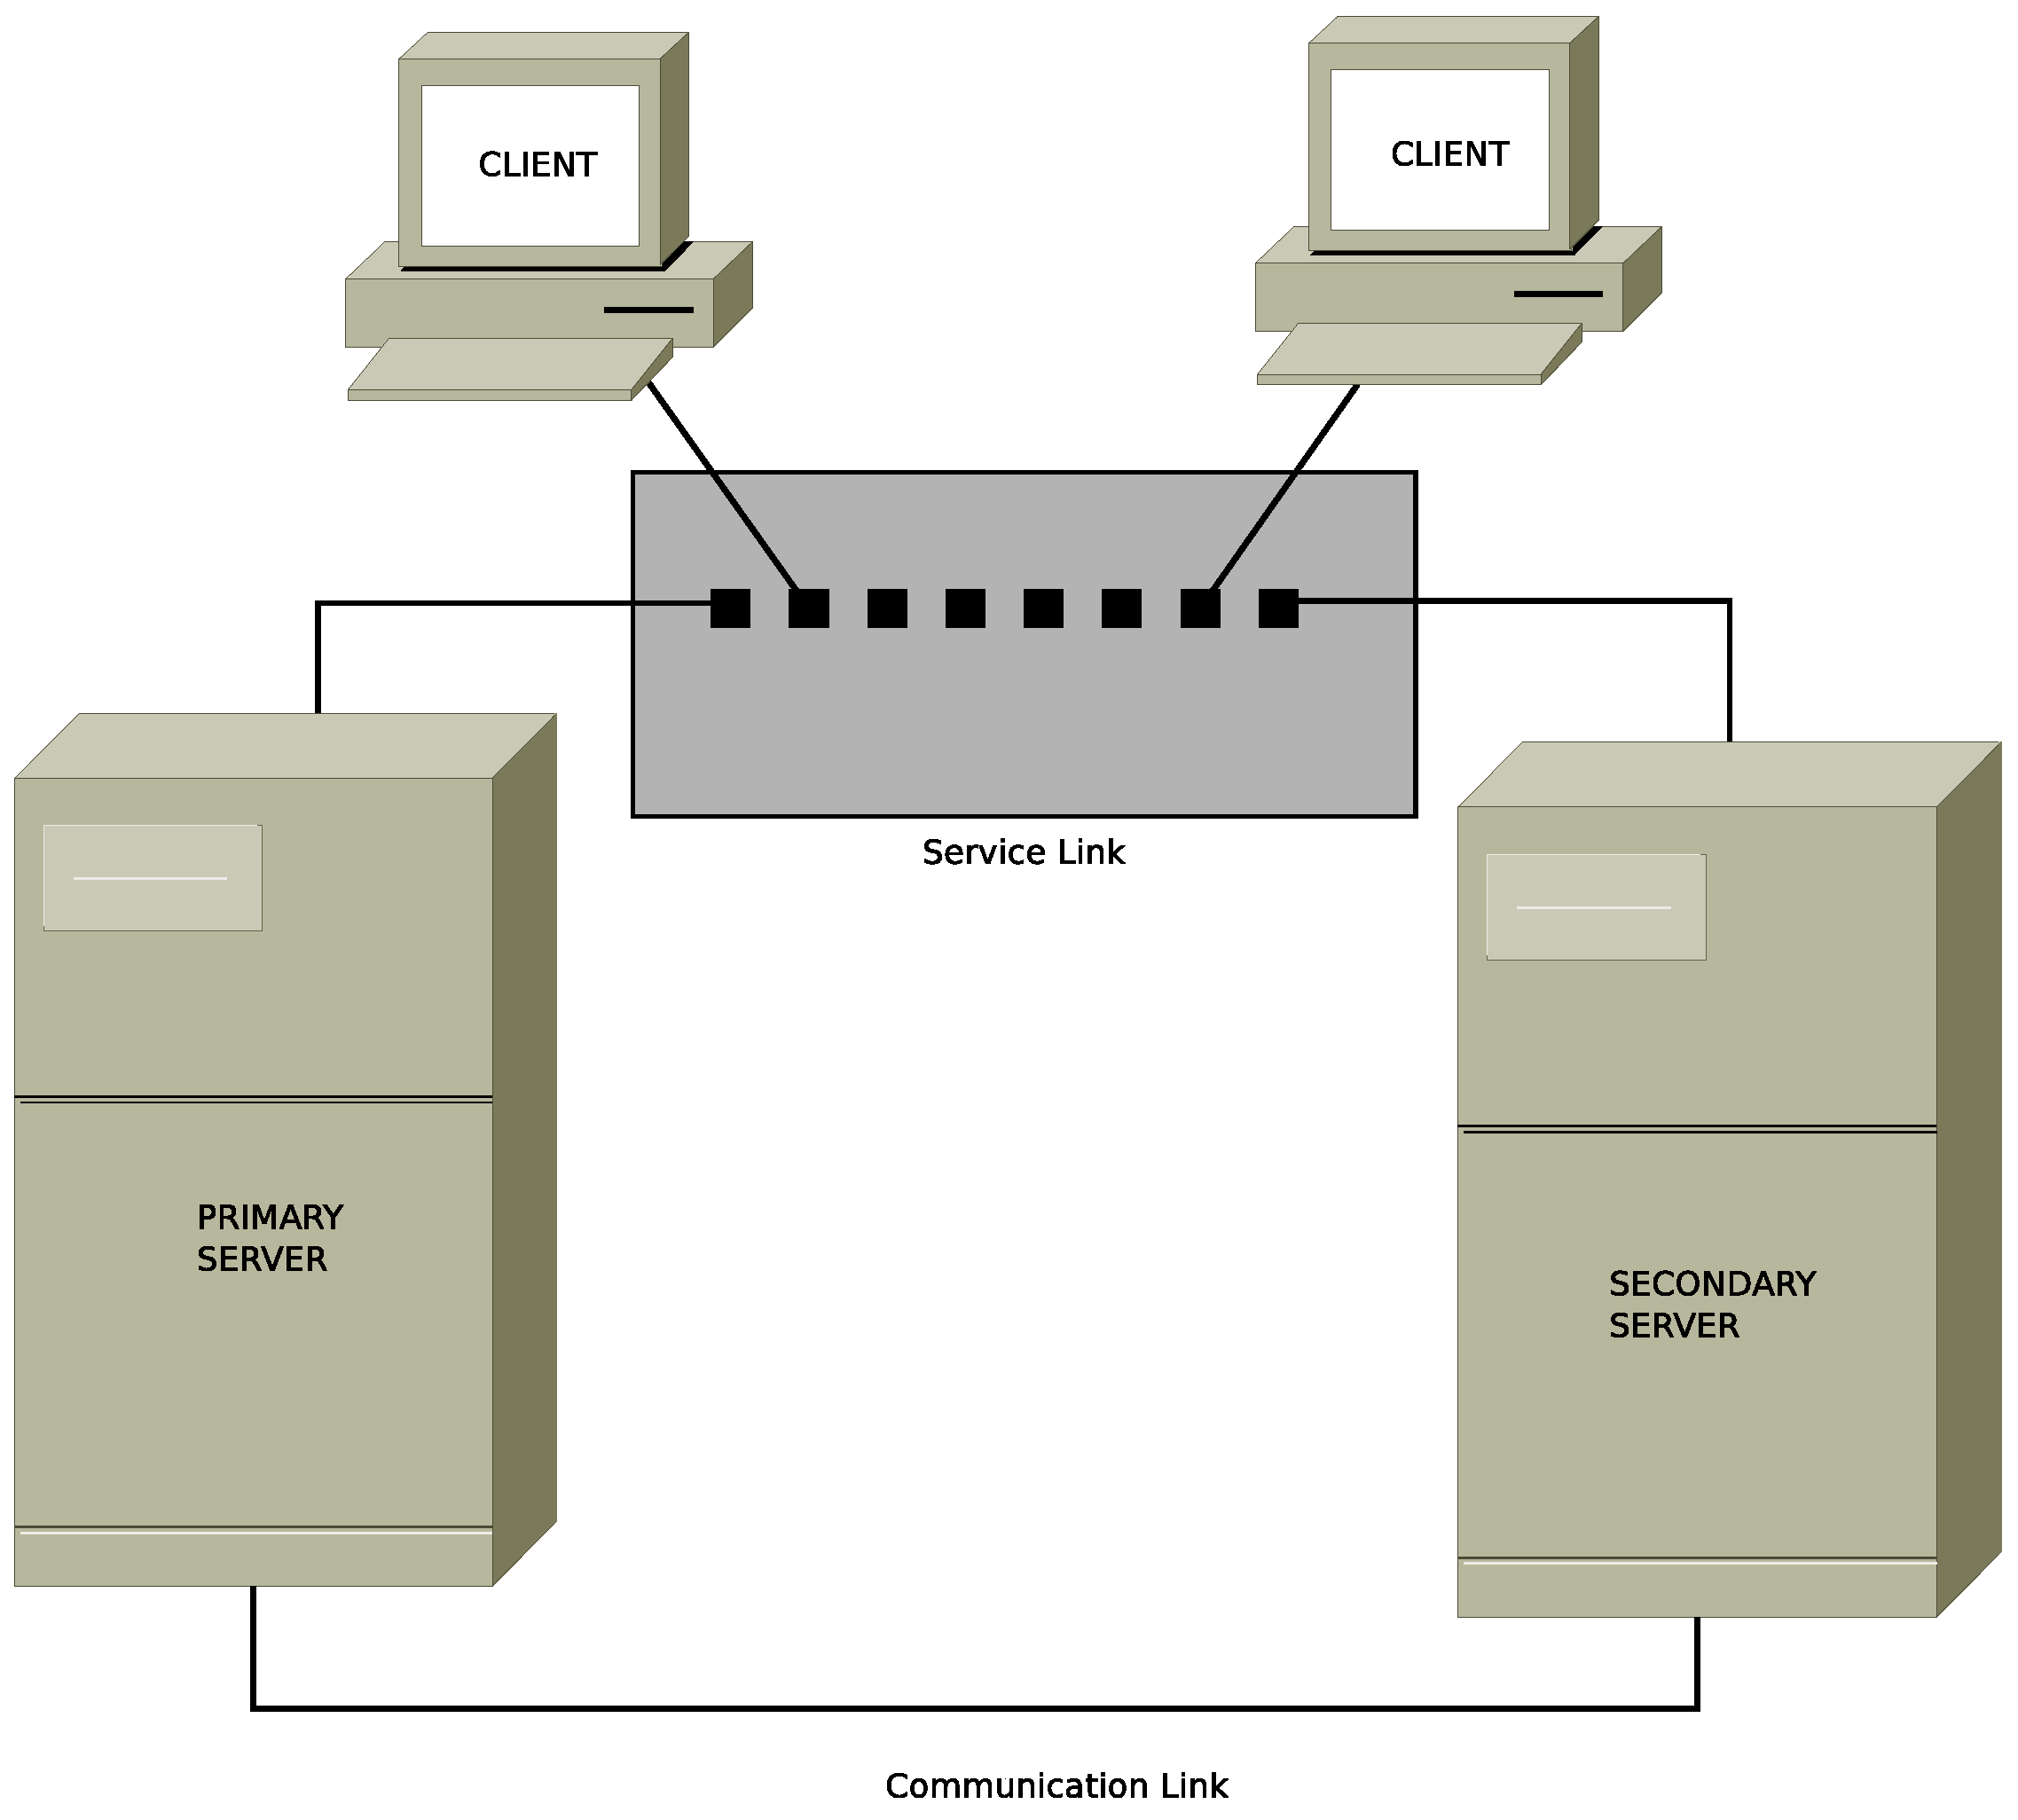
\includegraphics[scale=0.19,keepaspectratio=true]{./img/ha_main_schema.eps}
  % ha_main_schema.eps: 0x0 pixel, 300dpi, 0.00x0.00 cm, bb=0 0 1076 969
\end{center}


\end{frame}

\section {LAB}

\begin{frame}
\frametitle{LAB}

\begin{itemize}

\item  {Operating System Installation}
\item  {Network setup}
\item  {Zimbra installation}
\item  {DRBD Setup}
\item  {Disable Zimbra and DRBD startup scripts}
\item  {Corosync setup}
\item  {Zimbra OCF Resource Agent Development}
\item  {Pacemaker setup}

\end{itemize}
\end{frame}

\begin{frame}
\frametitle{LAB - Zimbra OCF Resource Agent Development (1/2)}

\begin{itemize}

\item  {OCF: Standardized interface for a cluster resource}
\item  {Cluster resource examples:
  \begin{itemize}
    \item IP address
    \item DRBD partition
    \item Filesystem mount
    \item Zimbra server
  \end{itemize}
}

\item Specific steps to the resource or application
\item  {Result: Success or Failure}


\end{itemize}
\end{frame}

\begin{frame}
\frametitle{LAB - Zimbra OCF Resource Agent Development (2/2)}

\begin{block}{}
bTactic Zimbra OCF Resource Agent actions
\end{block}

\begin{itemize}

  \item {\textbf{start . Starts the Zimbra resource}
    \begin{itemize}
      \item Exit 0 (Zimbra starts OK)
      \item Exit != 7 or Exit != 0 (Zimbra fails to start)
    \end{itemize}
  }
  \item {\textbf{stop . Stops the Zimbra resource}
    \begin{itemize}
      \item Exit 0 (Zimbra stops OK)
      \item Exit != 7 or Exit != 0 (Zimbra fails to stop)
    \end{itemize}
  }
  \item {\textbf{monitor . Monitors Zimbra resource health}
    \begin{itemize}
      \item Exit 0 (Zimbra is running)
      \item Exit 7 (Zimbra is stopped)
      \item Exit != 7 or Exit != 0 (Zimbra monitor has failed)
    \end{itemize}
  }
  \item {\textbf{meta-data} : Provide information about Zimbra resource as an XML snippet. Exit 0.}

\end{itemize}
\end{frame}

%\section {HA System Management}
\section {Live DEMO}

\begin{frame}

\frametitle{Zimbra HA Live DEMO}


\begin{center}
  \begin{itemize}
    \item Resources check with {\tt crm\_mon}
    \item Turn off active node
    \item Stop resources manually
  \end{itemize}
\end{center}




\end{frame}
\section {Future work}

\begin{frame}
\frametitle{Future work}

\begin{itemize}
  \item OVH Datacentre network handling
  \item Fencing
  \item Mysql HA
  \item Project Always ON
  \item Data Loss measurement
\end{itemize}
\end{frame}
\section {Conclusions}
\begin{frame}

\frametitle{Conclusions}


\begin{center}
  \begin{itemize}
    \item Shared storage thanks to DRBD
    \item State of the art HA software such as Pacemaker and Corosync has been used
    \item Active/Passive cluster implemented
    \item Zimbra HA with OSE version implemented
  \end{itemize}
\end{center}




\end{frame}

\end{document}
